
%%%%%%%%%%%%%%%%%%%%%%%%%%%%%%%%%%%%%%%%%%%%%%%%%%%%%%%%%%%%
\documentclass[xcolor=x11names,compress]{beamer}

\definecolor{CoolBlack}{rgb}{0.0, 0.18, 0.39}
\definecolor{byellow}{rgb}{0.55037, 0.38821, 0.06142}
%% General document %%%%%%%%%%%%%%%%%%%%%%%%%%%%%%%%%%
\usepackage{graphicx}
\usepackage{tikz}
\usepackage{Tabbing}
\usetikzlibrary{decorations.fractals}
%%%%%%%%%%%%%%%%%%%%%%%%%%%%%%%%%%%%%%%%%%%%%%%%%%%%%%

%% Beamer Layout %%%%%%%%%%%%%%%%%%%%%%%%%%%%%%%%%%
\useoutertheme[subsection=false,shadow]{miniframes}
\useinnertheme{default}
\usefonttheme{serif}
\usepackage{palatino}
\usepackage{tabu}

% addition of color
\usepackage{xcolor}
\definecolor{dgreen}{rgb}{0.,0.6,0.}
\definecolor{RawSienna}{cmyk}{0,0.72,1,0.45}

\setbeamerfont{title like}{shape=\scshape}
\setbeamerfont{frametitle}{shape=\scshape}

\setbeamercolor*{lower separation line head}{bg=CoolBlack} 
\setbeamercolor*{normal text}{fg=black,bg=white} 
\setbeamercolor*{alerted text}{fg=dgreen} 
\setbeamercolor*{example text}{fg=black} 
\setbeamercolor*{structure}{fg=black} 
 
\setbeamercolor*{palette tertiary}{fg=black,bg=black!10} 
\setbeamercolor*{palette quaternary}{fg=black,bg=black!10} 

% Links
\usepackage{hyperref}
\definecolor{links}{HTML}{003262}
\hypersetup{colorlinks,linkcolor=,urlcolor=links}

% columns
\renewcommand{\(}{\begin{columns}}
\renewcommand{\)}{\end{columns}}
\newcommand{\<}[1]{\begin{column}{#1}}
\renewcommand{\>}{\end{column}}

% adding slide numbers
\addtobeamertemplate{navigation symbols}{}{%
    \usebeamerfont{footline}%
    \usebeamercolor[fg]{footline}%
    \hspace{1em}%
    \insertframenumber/\inserttotalframenumber
}

% equation stuff
\newcommand{\Macro}{\ensuremath{\Sigma}}
\newcommand{\Sn}{\ensuremath{S_N} }
\newcommand{\vOmega}{\ensuremath{\hat{\Omega}}}
\usepackage{mathrsfs}
\usepackage[mathcal]{euscript}
\usepackage{amssymb}
\usepackage{amsthm}
\usepackage{epsfig}
\usepackage{amsmath}

\newcommand{\ve}[1]{\ensuremath{\mathbf{#1}}}
\newcommand{\micro}{\ensuremath{\sigma}}
\newcommand{\detR}{\ensuremath{\Sigma}}
%%%%%%%%%%%%%%%%%%%%%%%%%%%%%%%%%%%%%%%%%%%%%%%%%%

\begin{document}

%%%%%%%%%%%%%%%%%%%%%%%%%%%%%%%%%%%%%%%%%%%%%%%%%%%%%%
%%%%%%%%%%%%%%%%%%%%%%%%%%%%%%%%%%%%%%%%%%%%%%%%%%%%%%
\begin{frame}
\title{Solving Shielding Challenges:}
\subtitle{Self-Shielding and Strong Anisotropies}
\author{\includegraphics[height=2cm]
{../bk-eps-converted-to}\\R.\ N.\ Slaybaugh, UC Berkeley \\ S.\ C.\ Wilson, ORNL}
\date{11 June 2015 \\ Oak Ridge National Laboratory}
\titlepage
\end{frame}


% As you prepare your presentation, keep in mind that most of the students won’t have a radiation transport background so a couple slides on “what radiation transport is”, “why its needed”, and “where it’s used” would be nice :).

% --------------------------------------------------------------
\begin{frame}[fragile]{Outline}
  \frametitle{Outline}

\begin{columns}
  \begin{column}{0.6\textwidth}
    \begin{itemize}
    \item Hybrid methods overview
    \begin{itemize}
    		\item Motivation
		\item CADIS and FW-CADIS
		\item Challenges
    \end{itemize}
    	\item MC importances with space and energy self-shielding
	\begin{itemize}
    		\item Cross section processing
		\item Problem investigation
		\item Resonance factor method
		\item Results and wrap-up
  	\end{itemize}
	\item MC importances with strong anisotropies
  \end{itemize}
  \end{column}
  \begin{column}{0.4\textwidth}
  	\begin{figure}
  	\begin{center}
  		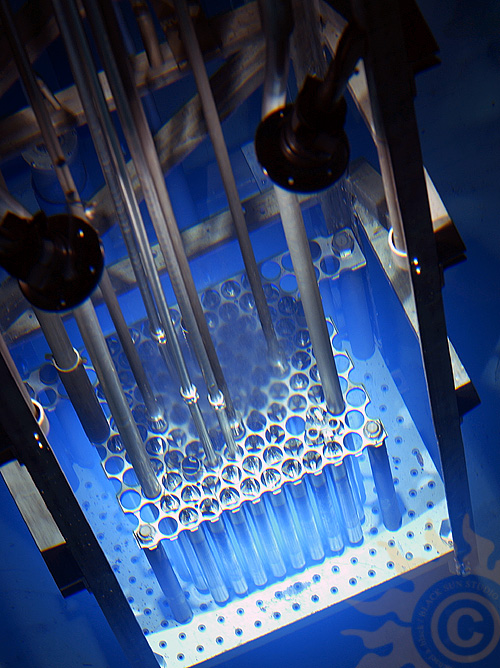
\includegraphics[height=2in,clip]{../figs/psu-reactor}
	\end{center}
  	\end{figure}
  \end{column}
\end{columns}

\end{frame}

% --------------------------------------------------------------
% --------------------------------------------------------------
\section{\scshape Hybrid Methods}
%\subsection{Motivation}
\begin{frame}[fragile]
  \frametitle{Project motivation}

\begin{columns}
  \begin{column}{0.55\textwidth}
	\begin{itemize}
	\item Need to accurately model radiation for shielding
	\item \alert{Challenging}: dense shields; streaming paths; multigroup x-secs
	\item Current methods are insufficient
	\item \alert{Goal}: accurate solutions in reasonable time
	\end{itemize}
  \end{column}
  \begin{column}{0.45\textwidth}
  	\begin{figure}
  	\begin{center}
  		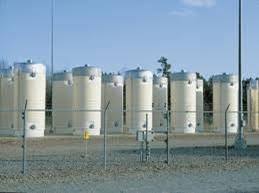
\includegraphics[height=1.25in,clip]{../figs/isfsi}
		\caption{Used fuel storage pad}
	\end{center}
  	\end{figure}
  \end{column}
\end{columns}

\end{frame}


% --------------------------------------------------------------
% --------------------------------------------------------------
%\section{\scshape Hybrid Methods}
%\subsection{Motivation}
\begin{frame}[fragile]
  \frametitle{Boltzmann transport equation}

\textit{Where} are all the neutrons? \textit{Why} do we care?
\pause
\begin{align}
\vOmega \cdot \nabla \psi(\vec{r}, E, \vOmega) &+
\Sigma_t \psi(\vec{r}, E, \vOmega) = S(\vec{r}, E, \vOmega) \:+\nonumber\\
%
& \int_{4\pi} d\vOmega' \int_0^{\infty} dE'\: \Sigma_s(E', \vOmega' \rightarrow E, \vOmega) \psi(\vec{r}, E', \vOmega') \nonumber
\end{align}

\begin{itemize}
\item $\psi(\vec{r}, E, \vOmega)$ is the angular neutron flux in neutrons per unit length squared per steradian,
\item $\Sigma$s are the probabilities of interaction (total or scattering) with units of inverse length, and
\item $S(\vec{r}, E, \vOmega)$ is a fixed source
\end{itemize}

\end{frame}

% --------------------------------------------------------------
\begin{frame}[fragile]
  \frametitle{Solving the TE}
%
\begin{columns}
  \begin{column}{0.5\textwidth}
  \begin{center}
  \underline{Monte Carlo}
  \end{center}
	\begin{itemize}
	\item Solution has statistical error
	\item \textit{Continuous} phase space: ``gold standard answers"
	\item Long compute times
	\item Optically thick = \textit{slow}
	\item Good for streaming
	\end{itemize}
  \end{column}
  \begin{column}{0.5\textwidth}
  \begin{center}
  \underline{Deterministic}
  \end{center}
	\begin{itemize}
	\item Solution equally valid everywhere
	\item \textit{Discretized} phase space: drives solution quality
	\item Can be fast
	\item Streaming = \textit{ray effects}
	\item Good for optically thick
	\end{itemize}
  \end{column}
\end{columns}

\end{frame}


% --------------------------------------------------------------
\begin{frame}[fragile]
  \frametitle{Speeding up MC}
  \begin{itemize}
  	\item To use MC in many applications, we need to \alert{improve} it
	\item Variance reduction is designed to increase the FOM:
  \end{itemize}
\begin{align}
\text{FOM} = \frac{1}{\text{R}^2\text{t}}\:,
 \qquad & \text{R = relative error} \nonumber \\ 
& \text{t = time} \nonumber 
\end{align}
  \begin{itemize}
  \pause
  	\item \underline{Idea}: can we use deterministic and Monte Carlo methods together to lessen the weaknesses of each?
  \end{itemize}
  \pause
  $\rightarrow$ \textbf{Hybrid Methods}

\end{frame}


% --------------------------------------------------------------
%\subsection{CADIS}
\begin{frame}[fragile]
  \frametitle{Forward-adjoint relationship}
Define response with function $f(\ve{r}, E)$ in volume $V_r$ as
%
\begin{equation}
 R = \int_E \int_{V_r} f(\ve{r}, E) \phi(\ve{r}, E) dV dE 
 \label{eq:Response}
\end{equation}\pause
%
\begin{columns}
  \begin{column}{0.5\textwidth}
	\begin{align}
  	H\phi &= q \quad \text{(forward)}\nonumber \\
  	%
  	H^{\dagger} \phi^{\dagger} &= q^{\dagger} \quad 
  	\text{(adjoint)}\nonumber
  	\end{align}
  \end{column}
  \begin{column}{0.5\textwidth}
  	\begin{align}
  	\langle H\phi, \phi^{\dagger} \rangle &= \langle H^{\dagger} \phi^{\dagger}, \phi \rangle \:, \text{and therefore} \nonumber \\
  	%
  	\langle q, \phi^{\dagger} \rangle &= \langle q^{\dagger}, \phi \rangle \nonumber
  	\end{align}
  \end{column}
\end{columns}
\vspace*{1 em}
\pause
If we let $q^{\dagger} = f(\ve{r}, E)$, then
%
\begin{equation}
 \langle q^{\dagger}, \phi \rangle = \langle f, \phi \rangle = R = \langle q, \phi^{\dagger} \rangle
 \label{eq:ResponseRedef}
\end{equation}
%
Eq.\ \eqref{eq:ResponseRedef} expresses that $\phi^{\dagger}$ represents the expected contribution of a source particle to the response.

\end{frame}


% --------------------------------------------------------------
\begin{frame}[fragile]
  \frametitle{CADIS \cite{Wagner2007}}
  
  \begin{enumerate}
  \item Define $q^{\dagger}$ as the local response of interest\\
  \item Coarse deterministic calculation to get $\phi^{\dagger}$ and $R$
  \end{enumerate}
% 
\begin{align*}
  imp(\ve{r}, E) &= \frac{\phi^{\dagger}(\ve{r}, E)}{\langle q(\ve{r}, E), \phi^{\dagger}(\ve{r}, E) \rangle} = \frac{\phi^{\dagger}(\ve{r}, E)}{R} \\
  %
  \hat{q}(\ve{r}, E) &= \frac{\phi^{\dagger}(\ve{r}, E) q(\ve{r}, E)}{R} \\
  %
  w_0(\ve{r}, E) &= \frac{q(\ve{r}, E)}{\hat{q}(\ve{r}, E)} = \frac{R}{\phi^{\dagger}(\ve{r}, E)} 
  \label{eq:Importance}
\end{align*}

Birth weights match weight targets: \underline{C}onsistent \underline{A}djoint \underline{D}riven \underline{I}mportance \underline{S}ampling \underline{M}ethod

\end{frame}


% --------------------------------------------------------------
%\subsection{FW-CADIS}
\begin{frame}[fragile]
  \frametitle{FW-CADIS \cite{Wagner2007}}

\begin{itemize}
\item We often what to optimize solutions in all of phase space\\
\item In this case the adjoint source needs to be a global forward solution: \underline{F}orward \underline{W}eighted-CADIS
\end{itemize}\pause
%
\begin{columns}
  \begin{column}{0.5\textwidth}
  \begin{center}
  \alert{To Optimize}
  \end{center}
	\begin{align}
  	&\phi(\ve{r}, E)\nonumber \\
  	%
  	\int&\phi(\ve{r}, E)\sigma_d(\ve{r}, E)\nonumber
  	\end{align}
  \end{column}
  %
  \begin{column}{0.5\textwidth}
  \begin{center}  
  \alert{Adjoint Source}
  \end{center}
  	\begin{align}
  	f(\ve{r}, E) &= \frac{1}{\phi(\ve{r}, E)}\nonumber \\
  	%
  	f(\ve{r}, E) &= \frac{\sigma_d(\ve{r}, E)}{\int\phi(\ve{r}, E)\sigma_d(\ve{r}, E)} \nonumber
  	\end{align}
  \end{column}
\end{columns}
\vspace*{1 em}
For example
%
\begin{equation}
 R = \int_E \int_{V_f} f(\ve{r}, E) \phi(\ve{r}, E) dV dE = \int_E \int_{V} \frac{1}{\phi(\ve{r}, E)} \phi(\ve{r}, E) dV dE \approx 1 \nonumber
\end{equation}

\end{frame}


% --------------------------------------------------------------
%\subsection{Challenges}
\begin{frame}[fragile]
  \frametitle{Challenges}

	FW-CADIS works well for \textbf{most} shielding problems...
	%
	\begin{columns}
  	\begin{column}{0.5\textwidth}
  	\begin{figure}
  	\begin{center}
  		\includegraphics[height=1.9in,clip]{../figs/dlvn}
		\caption{Dog Legged Void Neutron shielding benchmark}
	\end{center}
  	\end{figure}
  	\end{column}
 	%
 	\begin{column}{0.5\textwidth}
 	\begin{figure}
  	\begin{center}
  		\includegraphics[height=1.9in,clip]{../figs/dlvn-lowVR}
  		\caption{MC 95\% CI RE using FW-CADIS, DLVN \cite{Slaybaugh2013}}
  	\end{center}
  	\end{figure}
  	\end{column}
	\end{columns}
  
\end{frame}


% --------------------------------------------------------------
\begin{frame}[fragile]
  \frametitle{Challenges}

	...but not \textbf{all} of them
	%
	\begin{columns}
  	\begin{column}{0.45\textwidth}
  	\begin{center}
  	\begin{figure}
  		\includegraphics[height=2in,clip]{../figs/plate-badVR}
  		\caption{MC 95\% CI RE using FW-CADIS, plate \cite{Wilson2015}}
  	\end{figure}
	\end{center}
  	\end{column}
 	%
 	\begin{column}{0.5\textwidth}
  	\begin{center}
  	\begin{itemize}
  		\item An example case: 
		\begin{itemize}
		    \item Energy self-shieding + 
		    \item Spatial self-shielding
		\end{itemize}
		\item High relative error through location of interest \vspace*{0.5 em}
		\pause
		\item FW-CADIS only includes space and energy, \textit{not angle} \vspace*{0.5 em}
		\pause
		\item We're also using multigroup x-secs
	\end{itemize}
  	\end{center}
  	\end{column}
	\end{columns}

\end{frame}


% --------------------------------------------------------------
%% --------------------------------------------------------------
\section{\scshape Self-Shielding}
%\begin{frame}[fragile]
%  \frametitle{Self-shielding (quick aside)}
%
%	\begin{itemize}
%	\item \underline{Spatial self-shielding} occurs at interface locations between materials with different absorption/transport properties. There is a reduction in flux in the absorbing material, which results in fewer total absorptions in that spatial location; the location \textit{shields} itself. \vspace*{1em}
%	
%	\item \underline{Energy self-shielding} occurs at resonance peaks. There is a reduction in flux due to the large absorption cross section. This results in fewer total absorptions over that energy range (flux is depressed). Thus, the resonance peak \textit{shields} itself.
%%Reference https://www.physicsforums.com/threads/energy-self-shielding.724795/
%	\end{itemize}
%
%\end{frame}


% --------------------------------------------------------------
%\subsection{Cross Section Processing}
\begin{frame}[fragile]
  \frametitle{Cross section processing \cite{Bondarenko1964}}

	\begin{itemize}
	\item General Case
	\begin{equation}
  	\micro_{x,g}^{(j)} = \frac{\langle \micro_x^{(j)}(u) W(u)\rangle}
	{\langle W(u)\rangle} \:, \quad W(u) = \phi_{\infty}(u) \nonumber
 	 \label{eq:baseBondarenko}
 	\end{equation} 
 	
 	\pause
 	\item Bondarenko method uses a background cross section
 	\begin{equation}
  	\micro_0^{(j)} = \frac{1}{N_j} \sum_{m \ne j} \micro_{t}^{(m)} N_m 
  	%\label{eq:bgxsec}
  	\:, \quad \micro_{x,g}^{(j)}(\micro_0^{(j)}) = \frac{\langle
  	 \micro_{x}^{(j)}(u) \frac{\phi_{\infty}(u)} {\micro_{t}^{(j)}(u)
  	 + \micro_0^{(j)}} \rangle}
  	 { \langle \frac{\phi_{\infty}(u)}{\micro_{t}^{(j)}(u) +
  	 \micro_0^{(j)}}\rangle} \nonumber
  \label{eq:ssfact}
	\end{equation}
	\item W(u) changed to include the  spectral difference assumption and effect of other isotopes
	\end{itemize}
	
\end{frame}
	
	
% --------------------------------------------------------------
\begin{frame}[fragile]
  \frametitle{Cross section processing}

	\begin{itemize}
	\item When a nuclide is dilute, $\sigma_0^{(j)} >>
	 \sigma_t^{(j)}$, $W(u) \rightarrow$ uncorrected 
		\begin{itemize}
		\item Large $\sigma_0$ = infinitely dilute case	
		\end{itemize}

	\item When a nuclide is concentrated, $\sigma_0^{(j)} << 
	 \sigma_t^{(j)}$, resonances have a larger impact 
		\begin{itemize}
		\item Small $\sigma_0$ = resonance case	
		\end{itemize}
	\end{itemize}

    \pause	
	\begin{itemize}
	\item Add correction for `thin slab' of resonance material in 
	`thick slab' of moderator
	\begin{align}
  	&\sigma_0^{*,(j)} = \frac{1}{N_j} \sum_{m \ne j} \sigma_{t}^{(m)} N_m 
	+ \frac{1}{N_j \bar{l}} \nonumber\\
  	&\text{\textcolor{byellow}{thin slab:}}\:\bar{l} \approx \frac{4V}{S} \qquad \text{\textcolor{byellow}{no effect:}}\:\bar{l} \approx \text{large} \nonumber
	\end{align}
	\end{itemize}
  
\end{frame}


% --------------------------------------------------------------
%\subsection{Problem Investigation}
\begin{frame}[fragile]
  \frametitle{Problem investigation}
  	\begin{columns}
  	\begin{column}{0.4\textwidth}
  	\begin{figure}
  		\includegraphics[height=2in,clip]{../figs/plate-geometry}
  		\caption{Shielding Stack Up}
  	\end{figure}
  	\end{column}
 	%
 	\begin{column}{0.6\textwidth}
	\begin{itemize}
	\item 53 cm $\times$ 50 cm $\times$ 140 cm 
	\item Uniform in x except plate (25-28 cm in x; 30-130 cm in z)
	\item Uniform in y
	\item U-235 fission spectrum; homogenized U, Zr, and H2O
	\vspace*{1 em}
	\item MC21, MCNP, and PARTISN
	\item ENDF/B-VII data (all codes)
	\item Processed by TRANSX (multigroup)
	\end{itemize}
  	\end{column}
	\end{columns}
  
\end{frame}


% --------------------------------------------------------------
\begin{frame}[fragile]
  \frametitle{Base calculation parameters}
  \begin{table}[p]
  \label{tab:calcParams}
  \begin{center}
    \begin{tabu}{| X | X | X |}\hline
      Variable & PARTISN & MC21\\\hline\hline
	Deterministic Mesh & 0.5 cm unif; 0.25 cm in x over 24 to 29 cm & 1 cm uniform \\\hline
	Tally mesh & N/A & 1 cm uniform \\\hline
	N particles & N/A & $1 \times 10^{10}$\\\hline
	Energy structure & 58 grps & 27 grps / cont.\\\hline
	Angular quad & QR-18-252 & QR-8-36\\\hline
	Scattering order & $P_3$ & $P_3$\\\hline
	Convergence & 0.01 & 0.05\\\hline
	TRANSX settings & $\bar{l}$ = 10,000 & $\bar{l}$ = 10,000\\\hline
	Dose Conv.\ Facs. & 58 grps & 27 grps \\\hline
    \end{tabu}
  \end{center}
\end{table}
  
\end{frame}


% --------------------------------------------------------------
\begin{frame}[fragile]
  \frametitle{Errors in plate}
 \begin{figure}[p]
   \begin{center}
     \includegraphics[height=2 in,clip]{../figs/NSE13-109R1-PlateDRandRE}
   \end{center}
   \caption{Base-case FW-CADIS MC21 dose rate (left) and 95CI RE (right) (xz-slice through y=25 cm)}
   \label{fig:Plate}
 \end{figure}
\end{frame}


%% --------------------------------------------------------------
%\begin{frame}[fragile]
%  \frametitle{Correct Without Plate}
% \begin{figure}[p]
%   \begin{center}
%     \includegraphics[height=2in,clip]{../figs/NSE13-109R1-NoPlateDRandRE}
%   \end{center}
%   \caption{No-Plate MC21 dose rate (left) and 95CI RE (right) (xz-slice through y=25 cm)}
%   \label{fig:noPlate}
% \end{figure}
%\end{frame}


% --------------------------------------------------------------
\begin{frame}[fragile]
  \frametitle{Deterministic MC mismatch}
 \begin{figure}[p]
   \begin{center}
     \includegraphics[width=3.8in,clip]{../figs/NSE13-109R1-PlateFluxExcel}
   \end{center}
   \caption{Plate non-thermal flux (left axis) and method ratios (right axis) down the x-y centerline}
   \label{fig:PlateFlux}
 \end{figure}
\end{frame}


% --------------------------------------------------------------
\begin{frame}[fragile]
  \frametitle{Correct without plate}
 \begin{figure}[p]
   \begin{center}
     \includegraphics[width=3.8in,clip]{../figs/NSE13-109R1-NoPlateFluxExcel}
   \end{center}
   \caption{Plate non-thermal flux (left axis) and method ratios (right axis) down the x-y centerline}
   \label{fig:noPlateFlux}
 \end{figure}
\end{frame}


% --------------------------------------------------------------
\begin{frame}[fragile]
  \frametitle{Deterministic MC mismatch}
 \begin{figure}[p]
   \begin{center}
     \includegraphics[width=3.8in,clip]{../figs/NSE13-109R1-PlateExitSpectra}
   \end{center}
   \caption{Plate flux spectra (left axis) and PARTSN/MC21 (right axis) at start of air region (z = 130.5 cm)}
   \label{fig:PlateExit}
 \end{figure}
\end{frame}


% --------------------------------------------------------------
\begin{frame}[fragile]
  \frametitle{Investigation}

	\begin{itemize}
	\item Parameters
	\begin{tabbing}
	* Mean chord length: \hspace*{2em} \= $\bar{l} = \frac{4V}{S}$ vs.\ $\bar{l} = 10,000$ \\
	* Angular quadrature: \> CMG-591 vs.\ QR-18-252 \\
	* Scattering expansion: \> P$_{5}$ vs.\ P$_{3}$ \\
	* Importance mesh: 	\> 0.25 cm (x), 0.5 cm (y,z) \\ \> in plate vs. 1 cm \\
	* Energy Structure: 	\> 58 vs.\ 27 groups
	\end{tabbing}
	
	\item CADIS in 2 cm area following plate
%	\end{itemize}
%	%
%	\begin{columns}
%  	\begin{column}{0.6\textwidth}
%	\begin{itemize}
	\item Physics
		\begin{itemize}
		\item Polyethylene follow-on
		\item Cr plate (diff.\ res.\ mat.)
		\item Air in plate (no res.\ mat.)
		\end{itemize}
	\end{itemize}
%  	\end{column}
%  	%
% 	\begin{column}{0.35\textwidth}
% 	\begin{align}
% 	\text{FOM}_{\min} &= \frac{1}{R_{\max}^2t} \nonumber \\
% 	\text{FOM}_{\max} &= \frac{1}{R_{\min}^2t} \nonumber
% 	\end{align}
% 	\end{column}
%	\end{columns}
  
\end{frame}


% --------------------------------------------------------------
\begin{frame}[fragile]
  \frametitle{Parameters results}
  
  	\begin{itemize}
  	\item Geometric chord length $\rightarrow$ PARTISN flux \textit{farther} from correct, especially in plate
  	\item Angular quadrature $\rightarrow$ \textit{no differences} with impact
	\item Scattering order $\rightarrow$ (nearly) \textit{no change}
  	\end{itemize}
  	
  \begin{center}
    \begin{tabu}{|l|r|r|r|r|r|r|}\hline
      Case & N & CPU-hrs & Max RE & Avg RE & Min F & Avg F\\\hline
      %%
Base      & 1e10 & 849.77    & 0.810 & 1.02e-2 & 1.79e-3 & 11.3\\
%
1e11 & 1e11 & 8,543.47  & 0.164 & 3.28e-3 & \alert{4.33e-3} & 10.9\\
%
58 g & 1e10 & 954.89    & 0.522 & 9.33e-3 & \alert{3.85e-3} & 12.0\\
%
Fine & 1e10 & 905.34    & 1.55  & 1.71e-2 & 4.63e-4 & 3.78\\
%
F2e11 & 2e11 & 18,367.67 & 0.343 & 4.00e-3 & 4.62e-4 & 3.40\\\hline
    \end{tabu}
  \end{center}

\end{frame}


% --------------------------------------------------------------
\begin{frame}[fragile]
  \frametitle{CADIS, poly follow}
 \begin{figure}[p]
   \begin{center}
     \includegraphics[width=3.8in,clip]{../figs/cadis-poly}
   \end{center}
 \end{figure}
\end{frame}


% --------------------------------------------------------------
\begin{frame}[fragile]
  \frametitle{Resonance streaming}
   \begin{figure}[p]
   \begin{center}
     \includegraphics[width=3.8in,clip]{../figs/NSE13-109R1-CrAir}
   \end{center}
   \caption{Cr plate (left) and air plate (right) FW-CADIS MC21 dose rate 95CI RE (xz-slice through y=25 cm)}
   \label{fig:CrAir}
 \end{figure}
\end{frame}


% --------------------------------------------------------------
\begin{frame}[fragile]
  \frametitle{MAVRIC}
  
  \begin{itemize}
  \item We also ran this problem with and without the plate in MAVRIC (a multigroup MC code in SCALE)
  \item MAVRIC has more advanced cross section processing options
  \item Used 27 g and 200 g; in one 200 g case the plate had tailored x-secs every 10-cm \vspace*{0.5em}
  \pause
  \item Without plate case was correct
  \item 27 g $\rightarrow$ completely \textit{missed} the behavior
  \item Both 200 g cases $\rightarrow$ \textit{same} high relative error
  \end{itemize}
  
\end{frame}


% --------------------------------------------------------------
\begin{frame}[fragile]
  \frametitle{Investigation summary}
  
	\begin{itemize}
	\item Behavior is related to space and energy self-shielding
	\pause
	\item These items did not improve PARTISN:
	 \begin{itemize}
	 \item finer quadrature
	 \item higher scattering order
	 \item more theoretically-accurate mean chord length
	 \end{itemize}
	\pause 
	\item These items in imp.\ map creation did not reduce REs:
	 \begin{itemize}
	 \item finer spatial mesh in plate
	 \item finer energy group structure
	 \end{itemize}
	\pause 
	\item The high RE in and following the plate is present when using different codes and different methods to produce VR parameters, and exists when a different resonance material is used.
	\end{itemize}


A sufficiently accurate PARTISN solution would be better (probably), but prohibitively expensive.
  
\end{frame}


% --------------------------------------------------------------
%\subsection{Resonance Factor Method}
\begin{frame}[fragile]
  \frametitle{Resonance factor method \cite{Wilson2015}}
  	Apply renormalization factor to FW-CADIS source $q^{\dagger}_{FWC}$: 
	%
	\begin{equation}
   	q^{\dagger}(\ve{r},E) = \Bigl(\frac{\phi_{res(\micro_0)}(\ve{r},E)}{\phi_{dilute(\micro_0)}(\ve{r},E)}\Bigr)^M q^{\dagger}_{FWC}  \nonumber
  	 \label{eq:newQ}
	\end{equation}
	%
	where
	\begin{itemize}
  	\item M is problem-dependent constant 
 	 \item $\phi_{res(\micro_0)}(\ve{r},E)$ is forward flux with small background x-sec
 	 \item $\phi_{dilute(\micro_0)}(\ve{r},E)$ is forward flux with large background x-sec
	\end{itemize}
	\pause
	\vspace*{1 em}
	The resulting adjoint flux is used to make importances

	
	%Implementation: use $\phi_{res(\micro_0)}(\ve{r},E)$  in all locations where $\phi$ would be used in the FW-CADIS method
	
	
	
\end{frame}


%% --------------------------------------------------------------
%\begin{frame}[fragile]
%  \frametitle{Resonance factor method}
%  
%	Example: optimize the space- and energy-dependent flux
%	
%	\vspace*{1 em}
%	$q^{\dagger}_{FWC} = 1 / \phi$ and results in this corrected response: 
%	%
%	\begin{align}
% 	R &= \int_E \int_{V} \Bigl(\frac{\phi_{res(\micro_0)}(\ve{r},E)}{\phi_{dilute(\micro_0)}(\ve{r},E)}\Bigr)^M \frac{1}{\phi_{res(\micro_0)}(\ve{r}, E)} \phi_{res(\micro_0)}(\ve{r}, E) dV dE \nonumber
% 	\label{eq:newResponse} \\
%  	 &\approx \int_E \int_{V} \Bigl(\frac{\phi_{res(\micro_0)}(\ve{r},E)}{\phi_{dilute(\micro_0)}(\ve{r},E)}\Bigr)^M dV dE \nonumber
%	\end{align}
%	\pause
%	The expanded version of importance map in plate becomes:
%	%
%	\begin{equation}
% imp(\ve{r},E)= \frac{\phi_{res(\micro_0)}^{\dagger}(\ve{r},E)}{\int_E \int_{V} \bigl(\frac{\phi_{res(\micro_0)}(\ve{r},E)}{\phi_{dilute(\micro_0)}(\ve{r},E)}\bigr)^M dV dE} \nonumber
% 	 \label{eq:newImp}
%	\end{equation}  
%  
%\end{frame}


% --------------------------------------------------------------
%\subsection{Results}
\begin{frame}[fragile]
  \frametitle{Results}
    \begin{center}
  \includegraphics[width=4in,clip]{../figs/m1-vs-58g}  
  \end{center}
\end{frame}


% --------------------------------------------------------------
\begin{frame}[fragile]
  \frametitle{Results}

	\begin{table}[p]
 	 \label{tab:comparison}
  	\begin{center}
    \begin{tabular}{|l|r|r|r|r|r|}\hline
      Case & CPU-hrs & Max RE & Avg RE & Min FOM & Avg FOM\\\hline
      %%
base & 849.77 & 0.810 & 1.02e-2 & 1.79e-3 & 11.3\\
%
58 g & 954.89 & 0.522 & 9.33e-3 & 3.85e-3 & 12.0\\
%
M = 1 & \alert{534.80} & 0.269 & 2.44e-2 & \alert{2.58e-2} & 3.13\\\hline
    \end{tabular}
 	 \end{center}
	\end{table}

	\begin{itemize}
	\item M = 1.0 used same deterministic parameters as base case
	\item FOM$_{\min}$ $\sim$10x better than best FW-CADIS case
	\item FOM$_{\min}$ and FOM$_{\text{avg}}$ are $\sim$100x closer together than best FW-CADIS case
	\end{itemize}

\end{frame}


% --------------------------------------------------------------
%\subsection{Summary and Conclusions}
\begin{frame}[fragile]
  \frametitle{Resonance factor wrap-up}
  
  \begin{itemize}
  \item Space and energy self-shielding make VR difficult
  
  \item Caused by multigroup x-secs in angle-independent implementation
  
  \item Not resolved by
   \begin{itemize}
   \item Finer spatial mesh, energy group structure, or angular quadrature; higher order scattering expansion; or Bondarenko method
   \end{itemize}
  \pause 
  \item New method
   \begin{itemize}
  	\item Adds a factor accounting for resonances to FW-CADIS adjoint source
  	\item Tunable based on degree of problem manifestation
	\item \alert{Lowers FOM$_{\min}$ and brings FOM$_{\min}$ closer to FOM$_{\text{avg}}$}
	\item More work, but useful in these pathological cases
   \end{itemize}
  \end{itemize}

\end{frame}


% --------------------------------------------------------------
% --------------------------------------------------------------
\section{\scshape Strong Anisotropies}
\begin{frame}[fragile]
  \frametitle{Anisotropy: a computational challenge}

	\begin{columns}
  	\begin{column}{0.5\textwidth}
	\begin{itemize}
	\item Many important nuclear applications have strong anisotropies:
	 \begin{itemize}
	 \item Used fuel casks
	 \item Reprocessing facilities
	 \item Reactor facilities
	 \item Active interrogation 
	 \end{itemize}
	\pause
	\item Difficult to capture with current tools:
	 \begin{itemize}
	 \item Ray effects with deterministic
	 \item Too slow with analog MC
	 \item Insufficient acceleration of MC with current hybrid
	 \end{itemize}
	\end{itemize}
  	\end{column}
 	%
 	\begin{column}{0.5\textwidth}
 	 \begin{center}
 	 \begin{figure}
 	 \includegraphics[height=2in,clip]{../figs/pwr}  
 	 \caption{PWR relative error \cite{Pantelias2013}}
 	 \end{figure}
 	 \end{center}

  	\end{column}
	\end{columns}

\end{frame}


% --------------------------------------------------------------
\begin{frame}[fragile]
  \frametitle{Current hybrid methods are insufficient}

	\begin{itemize}
	\item MC VR parameters created from adjoint deterministic scalar flux that is a function of \textit{space and energy only} \vspace*{1 em}
	\item Angular dependence of the importance function is not retained, otherwise the map would be 
	\begin{itemize}
	  \item very large (tens or hundreds of GB) and
	  \item  more costly and complex to use in the MC simulation 
	\end{itemize}
	\item Drawback: within a given space/energy cell, the map provides the average importance of a particle moving in \textit{any direction} through the cell -- excluding information about how particles move \alert{toward the objective}
	\end{itemize}

\end{frame}


% --------------------------------------------------------------
\begin{frame}[fragile]
  \frametitle{Current hybrid methods are insufficient}

	\begin{columns}
  	\begin{column}{0.5\textwidth}
 	 \begin{center}
 	 \begin{figure}
 	 \includegraphics[height=2in,clip]{../figs/boat-interrogation}  
 	 \caption{Spherical boat model with source on left and fissionable material at center}
 	 \end{figure}
 	 \end{center}
  	\end{column}
 	%
 	\begin{column}{0.5\textwidth}
 	 \begin{center}
 	 \begin{figure}
 	 \includegraphics[height=2in,clip]{../figs/boat-map}  
 	 \caption{Target weight window values for 14.1 MeV neutrons}
 	 \end{figure}
 	 \end{center}
  	\end{column}
	\end{columns}

\end{frame}

% --------------------------------------------------------------
\begin{frame}[fragile]
  \frametitle{Many attempts at resolution $\rightarrow$ \\ 
  \hspace*{3em} Limited Success}

	\begin{itemize}
	\item Automatic WW generator in MCNP \cite{MCNP2008}
	\item AVATAR \cite{vanRiper1997}
	%in many cases in which anisotropies are important, including angular information will improve calculation efficiency. However, these results also showed that the simple angular CADIS implementation is not accurate enough to provide the improvement necessary to be able to efficiently execute the used fuel cask calculations we would like to perform to improve facility monitoring design and operation. 
	\item LIFT \cite{Turner1997}
	%derived from the zero-variance method and  uses an approximation of the adjoint flux that is piecewise continuous in angle. LIFT only captures linearly anisotropic scattering, which is not enough for our needs and is somewhat difficult to use
	\item Cooper and Larsen's global weight windows \cite{Cooper2001}
	\item FW/CADIS
	\item Resonance Factor method
	\end{itemize}
    All of these have worked in \textit{some} situations\\
    They often require \textit{significant} user expertise	
	
    \vspace*{1 em}
    \underline{Better hybrid methods are needed}: \alert{two ideas}.

\end{frame}

% --------------------------------------------------------------
\begin{frame}[fragile]
  \frametitle{Integration weighting}

    Different integration plan captures angles in scalar flux creation	
	\begin{align*}
		\phi^{\dagger}(\ve{r},E) &= \int \psi^{\dagger}(\vOmega, 
		\ve{r},E) d\vOmega \qquad  \qquad \qquad \text{original}\\
		 %
		\phi^{\dagger}(\ve{r},E) &= \frac{\int \psi(\vOmega, \ve{r},E)
		 \psi^{\dagger}(\vOmega, \ve{r},E) d\vOmega}{\int \psi(\vOmega, 
		 \ve{r},E)  d\vOmega} \qquad \text{\alert{new}}
	\end{align*}
%Note that these two calculations can be completed concurrently. Then, the adjoint scalar fluxes will be computed by angularly integrating the product of the forward and adjoint angular fluxes to account for the directions in which the particles will actually be traveling at any given location/energy:
%will provide importance values that more accurately reflect the average importance of particles that will be transported in the final Monte Carlo calculation, yielding faster Monte Carlo run times.

    \pause
    Major challenges and areas of investigation:
	\begin{enumerate}
	\item Data storage and handling (many GBs)
	\item More, less, or differently sensitive to 
	  \begin{itemize}
	  \item quality of the discrete ordinates calculation?
	  \item ray effects?
	  \end{itemize}
	\end{enumerate}

\end{frame}

% --------------------------------------------------------------
\begin{frame}[fragile]
  \frametitle{Lagrange discrete ordinate equations}

    Use a formulation that is more flexible in the ways 
	it handles quadrature: new LDO equations \cite{Ahrens2014}
	\vspace*{1 em}
	
	\begin{itemize}
	\item Re-derivation of $S_N$ with an \alert{interpolatory quadrature framework}
	\item Allows evaluation at directions not on quadrature set
	\item Can use \alert{asymmetric angles}
	\item No need to store spherical harmonic moments
	\item May be useful for more accurately capturing strong anisotropies
	\end{itemize}

\end{frame}

% --------------------------------------------------------------
\begin{frame}[fragile]
  \frametitle{Method implementation}

  	\begin{itemize}
    \item The space- and energy-dependent importance map will be normalized and 
     source biasing parameters will be generated in the \alert{same ways} as
     the current implementation of FW/CADIS \vspace*{1 em}
	\item Immediately useful; widely applicable \vspace*{1 em}
	\item We will study both strategies and characterize the impact\vspace*{1 em}
	\item Will be available in SCALE \cite{SCALE} and ADVANTG \cite{Pantelias2013}
	\end{itemize}
	
\end{frame}


% --------------------------------------------------------------
% --------------------------------------------------------------
\section*{}
\begin{frame}[fragile]
  \frametitle{Questions?}
  \begin{center}
  \includegraphics[height=3in,clip]{../questions-comic}  
  \end{center}
  
\end{frame}

% --------------------------------------------------------------
\begin{frame}[allowframebreaks]{References}
	\bibliographystyle{unsrt}
	\bibliography{2015-04-uf}
\end{frame}

\end{document}
